\documentclass[9pt,twocolumn,twoside]{g3_article/gsag3jnl}

\articletype{gs} % article type
% {inv} Investigations
% {msr} Mutant Screen Reports
% {gs} Genomic Selection
% {goi} Genetics of Immunity 
% {gos} Genetics of Sex 
% {mp} Multiparental Populations

\title{Template for preparing your submission \\to G3: Genes|Genomes|Genetics using Overleaf}

\author[$\ast$,1]{Riley McDowell}
\author[$\dagger$]{David Grant}
%\author[$\ddagger$]{Author Three}
%\author[$\S$]{Author Four}
%\author[$\ast\ast$]{Author Five}

\affil[$\ast$]{Iowa State University, US}
\affil[$\dagger$]{Iowa State University, US}
%\affil[$\ddagger$]{Author three affiliation}
%\affil[$\S$]{Author four affiliation}
%\affil[$\ast\ast$]{Author five affiliation}

%For the authors' names, indicate different affiliations with the 
%symbols: $\ast$, $\dagger$, $\ddagger$, $\S$. After four authors
%, the symbols double, triple, quadruple, and so forth as required.

\keywords{ genomic prediction \\ deep learning \\ neural network \\ genomic selection \\ SNP }

\runningtitle{ Genomic Prediction with Deep Networks } % Goes into the footer.

\correspondingauthor{Corresponding Author HERE} % TODO: Who is this?

\begin{abstract}

Reduced costs for DNA marker technology coupled has generated a huge amount of
molecular data and greatly increased the options available to characterize lines 
in a breeding program. Concurrently, the field of machine learning has experienced
a resurgence of research into techniques to detect or "learn" patterns in noisy
data in a variety of technical applications. Here, we apply so called "deep learning"
techniques from current machine learning research in neural networks to 
genomic selection and phenotypic selection problems on standard published datasets. 
We compare the results of these algorithms to the bayesian and linear regression techniques
commonly employed today.


%The abstract should be written for people who may not read the 
%entire paper, so it must stand on its own.  The impression it makes usually determines 
%whether the reader will go on to read the article, so the abstract must be 
%engaging, clear, and concise.  In addition, the abstract may be the only part of the 
%article that is indexed in databases, so it must accurately reflect the 
%content of the article. A well-written abstract is the  most effective way to reach intended 
%readers, leading to more robust search, retrieval, and usage of the article. 
%
%Please see additional guidelines notes on preparing your abstract below.

%\begin{itemize}
%\item provide a synopsis of the entire article;
%\item begin with the broad context of the study, followed by specific background for the study;
%\item describe the purpose, methods and procedures, core findings and results, and conclusions of the study;
%\item emphasize new or important aspects of the research;
%\item engage the broad readership of G3 and be understandable to a diverse audience (avoid using jargon);
%\item be a single paragraph of less than 250 words;
%\item contain the full name of the organism studied;
%\item NOT contain citations or abbreviations.
%\end{itemize}

\end{abstract}

\setboolean{displaycopyright}{true}

\begin{document}

\maketitle
\thispagestyle{firststyle}
\logomark
\articletypemark
\marginmark
\firstpagefootnote
\correspondingauthoraffiliation{CORRESPONDING AUTHOR ADDRESS AND EMAIL}%Please insert the affiliation correspondence address and email for the corresponding author. The corresponding author should be marked with a `1' in the author list, as shown in the example.}
\vspace{-11pt}%

\noindent % Skip header for 'Introduction'.

Markers are useful because they can be associated with traits.
QTL mapping, most useful for traits with small number of contributing loci.
Not useful for early breeding program selection or phenotypic prediction.

Meuwissen et al. (2001) publishes paper on genomic selection using
simulated data demonstrating prediction of offspring performance
from genotypic data using mixed models and bayesian methods.
Bayesian methods are most accurate.

Technique is applied to animal breeding, then plant breeding,
both successfully. Several alternate methods used. 

Several articles publish data and genomic selection algorithms,
reporting the accuracy of each on the dataset. One includes 
simple artificial neural network.

Concurrently, artificial intelligence research is rebranded as machine
learning, and the popularity of the interdisciplinary field known as data science 
increases dramatically. Data scientists apply machine learning and statistics 
from a wide variety of domains including mathematics, physics, and 
computer science to non-scientific domains such as sales and marketing.

Overview of networks and award-winning performance in many domains \citep{schmidhuber2015}.



% For the introduction, authors should be mindful of the broad readership of the journal. The introduction should set the stage for the importance of the work to a generalist reader and draw the reader in to the specific study. The scope and impact of the work should be clearly stated.

Authors are encouraged to:

\begin{itemize}
\item cite the supporting literature completely rather than select a subset of citations;
\item provide important background citations, including relevant review papers (to help orient the non-specialist reader);
\item to cite similar work in other organisms.
\end{itemize}

\section*{Materials and Methods}

Manuscripts submitted to G3 should contain a clear description of the experimental design in sufficient detail so that the experimental analysis could be repeated by another scientist. If the level of detail necessary to explain the protocol goes beyond two paragraphs, give a short description in the main body of the paper and prepare a detailed description for supporting information.  For example, details would include indicating how many individuals were used, and if applicable how individuals or groups were combined for analysis. If working with mutants indicate how many independent mutants were isolated. If working with populations indicate how samples were collected and whether they were random with respect to the target population.

\subsection*{Statistical Analysis} 

Indicate which statistical analysis has been performed and describe the method and model applied. If many genes were examined simultaneously, or many phenotypes, a multiple comparison correction should be used to control the type I error rate, or a rationale for not applying a correction must be provided. The type of correction applied should be clearly stated. It should also be clear whether the p-values reported are raw, or after correction. Corrected p-values are often appropriate, but raw p-values should be available in the supporting materials so that others may perform their own corrections. 

\subsection*{Data Availability}

At the end of the Materials and Methods section, include a statement on reagent and data availability. Please read the Data and Reagent Policy before writing the statement. Make sure to list the accession numbers or DOIs of any data you have placed in public repositories. List the file names and descriptions of any data you will upload as supplemental information. The statement should also include any applicable IRB numbers. You may include specifications for how to properly acknowledge or cite the data.

For example: Strains are available upon request. File S1 contains detailed descriptions of all supplemental files. File S2 contains SNP ID numbers and locations. File S3 contains genotypes for each individual. Sequence data are available at GenBank and the accession numbers are listed in File S3. Gene expression data are available at GEO with the accession number: GDS1234. Code used to generate the simulated data is provided in file S4. 

\section*{Results and Discussion}

The results and discussion should not be repetitive. The results section should give a factual presentation of the data and all tables and figures should be referenced; the discussion should not summarize the results but provide an interpretation of the results, and should clearly delineate between the findings of the particular study and the possible impact of those findings in a larger context. Authors are encouraged to cite recent work relevant to their interpretations. Present and discuss results only once, not in both the Results and Discussion sections. It is sometimes acceptable to combine results and discussion. The text should be as succinct as possible. Heed Strunk and White's dictum: "Omit needless words!"

\section*{Additional guidelines}

\subsection*{Numbers} In the text, write out numbers nine or less except as part of a date, a fraction or decimal, a percentage, or a unit of measurement. Use Arabic numbers for those larger than nine, except as the first word of a sentence; however, try to avoid starting a sentence with such a number.

\subsection*{Units} Use abbreviations of the customary units of measurement only when they are preceded by a number: "3 min" but "several minutes". Write "percent" as one word, except when used with a number: "several percent" but "75\%." To indicate temperature in centigrade, use ° (for example, 37°); include a letter after the degree symbol only when some other scale is intended (for example, 45°K).

\subsection*{Nomenclature and Italicization} Italicize names of organisms even when  when the species is not indicated.  Italicize the first three letters of the names of restriction enzyme cleavage sites, as in HindIII. Write the names of strains in roman except when incorporating specific genotypic designations. Italicize genotype names and symbols, including all components of alleles, but not when the name of a gene is the same as the name of an enzyme. Do not use "+" to indicate wild type. Carefully distinguish between genotype (italicized) and phenotype (not italicized) in both the writing and the symbolism.

\section*{In-text Citations}

Add citations using the \verb|\citep{}| command, for example \citep{neher2013genealogies} or for multiple citations, \citep{neher2013genealogies, rodelsperger2014characterization}.

For examples of different references, please see the example bibliography file 
(accessible via the Project menu in the Overleaf editor). This contains examples 
of articles \citep{neher2013genealogies, rodelsperger2014characterization}, a 
book \citep{Sturtevent2001}, a book 
chapter 
XXXX-SKIPPED-XXXX
%\citep{Sturtevent2001chp7}
, ahead-of-print work \citep{Starita2015} and software \citep{Kruijer2015}.

\section*{Examples of Article Components}
\label{sec:examples}

The sections below show examples of different header levels, which you can use in the primary sections of the manuscript (Results, Discussion, etc.) to organize your content.

\section*{First level section header}

Use this level to group two or more closely related headings in a long article.

\subsection*{Second level section header}

Second level section text.

\subsubsection*{Third level section header:}

Third level section text. These headings may be numbered, but only when the numbers must be cited in the text. 

\section*{Figures and Tables}

Figures and Tables should be labelled and referenced in the standard way using the \verb|\label{}| and \verb|\ref{}| commands.

\subsection*{Sample Figure}

Figure \ref{fig:spectrum} shows an example figure.

\begin{figure}[htbp]
\renewcommand{\familydefault}{\sfdefault}\normalfont
\centering
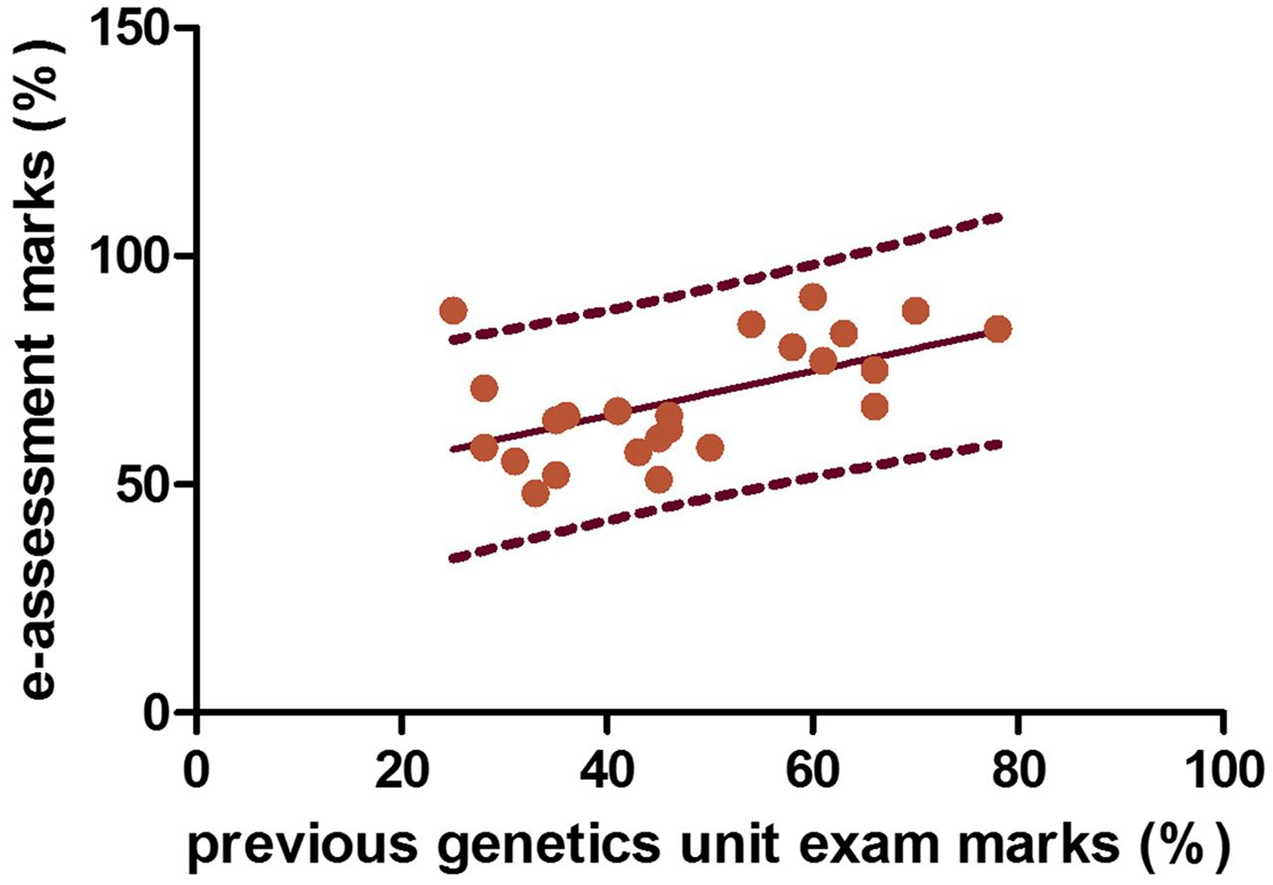
\includegraphics[width=\linewidth]{images/example-figure-g3}
\caption{Example figure from \url{http://dx.doi.org/10.1534/g3.115.017509}. Please include your figures in the manuscript for the review process. You can upload figures to Overleaf via the Project menu. Upon acceptance, we'll ask for your figure files to be uploaded in any of the following formats: TIFF (.tiff), JPEG (.jpg), Microsoft PowerPoint (.ppt), EPS (.eps), or Adobe Illustrator (.ai).  Images should be a minimum of 300 dpi in resolution and 500 dpi minimum if line art images.  RGB, CMYK, and Grayscale are all acceptable. Halftones should be high contrast with sharp detail, because some loss of detail and contrast is inevitable in the production process. Figures should be 10-20 cm in width and 1-25 cm in height. Graph axes must be exactly perpendicular and all lines of equal density.
Label multiple figure parts with A, B, etc. in bolded type, and use Arrows and numbers to draw attention to areas you want to highlight. Legends should start with a brief title and should be a self-contained description of the content of the figure that provides enough detail to fully understand the data presented. All conventional symbols used to indicate figure data points are available for typesetting; unconventional symbols should not be used. Italicize all mathematical variables (both in the figure legend and figure) , genotypes, and additional symbols that are normally italicized.  
}%
\label{fig:spectrum}
\end{figure}

\subsection*{Sample Video}

Figure \ref{video:spectrum} shows how to include a video in your manuscript.

\begin{figure}[htbp]
\renewcommand{\familydefault}{\sfdefault}\normalfont
\centering
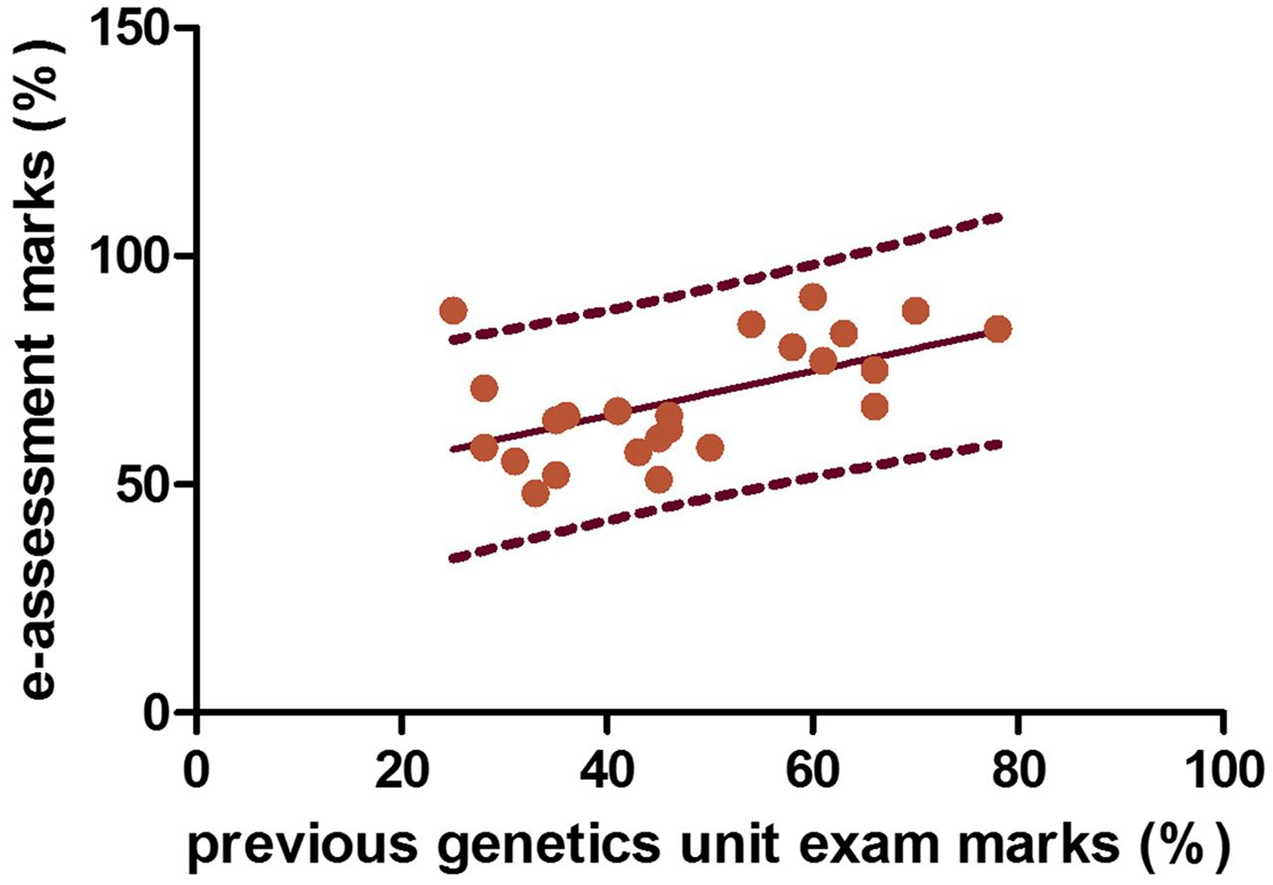
\includegraphics[width=\linewidth]{images/example-figure-g3}
\caption{Example movie (the figure file above is used as a placeholder for this example). G3 supports video and movie files that can be linked from any portion of the article - including the abstract. Acceptable formats include .asf, avi, .wav, and all types of Windows Media files.   
}%
\label{video:spectrum}
\end{figure}


\subsection*{Sample Table}

Table \ref{tab:shape-functions} shows an example table. Avoid shading, color type, line drawings, graphics, or other illustrations within tables. Use tables for data only; present drawings, graphics, and illustrations as separate figures. Histograms should not be used to present data that can be captured easily in text or small tables, as they take up much more space.  

Tables numbers are given in Arabic numerals. Tables should not be numbered 1A, 1B, etc., but if necessary, interior parts of the table can be labeled A, B, etc. for easy reference in the text.  


\begin{table*}[htbp]
\renewcommand{\familydefault}{\sfdefault}\normalfont
\centering
\caption{\bf Students and their grades}
\begin{tableminipage}{\textwidth}
\begin{tabularx}{\textwidth}{XXXX}
\hline
\header Student & Grade\footnote{This is an example of a footnote in a table. Lowercase, superscript italic letters (a, b, c, etc.) are used by default. You can also use *, **, and *** to indicate conventional levels of statistical significance, explained below the table.} & Rank & Notes \\
\hline
Alice & 82\% & 1 & Performed very well.\\
Bob & 65\% & 3 & Not up to his usual standard.\\
Charlie & 73\% & 2 & A good attempt.\\
\hline
\end{tabularx}
  \label{tab:shape-functions}
\end{tableminipage}
\end{table*}

\section*{Sample Equation}

Let $X_1, X_2, \ldots, X_n$ be a sequence of independent and identically distributed random variables with $\text{E}[X_i] = \mu$ and $\text{Var}[X_i] = \sigma^2 < \infty$, and let
\begin{equation}
S_n = \frac{X_1 + X_2 + \cdots + X_n}{n}
      = \frac{1}{n}\sum_{i}^{n} X_i
\label{eq:refname1}
\end{equation}
denote their mean. Then as $n$ approaches infinity, the random variables $\sqrt{n}(S_n - \mu)$ converge in distribution to a normal $\mathcal{N}(0, \sigma^2)$.

\bibliography{bibliography}

\end{document}
